% Q3: Toroidal Core — Physical cross-section with air gap and coil
% Uses TikZ (not CircuiTikZ) for geometric/physical drawing
\documentclass[border=10pt]{standalone}
\usepackage{tikz}
\usepackage{amsmath}
\usetikzlibrary{decorations.markings, patterns}
\renewcommand{\familydefault}{\sfdefault}

\begin{document}
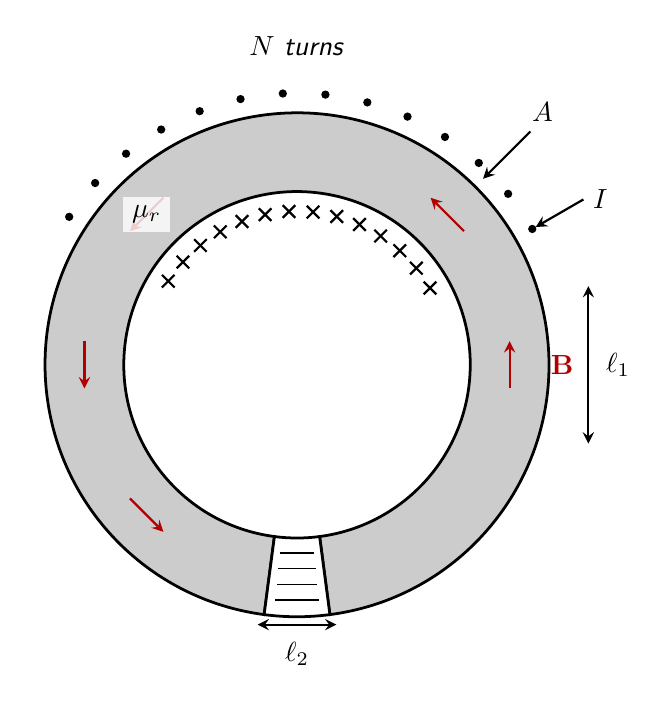
\begin{tikzpicture}[
    every node/.style={font=\sffamily},
    >=stealth
]

% Parameters
\def\Router{3.2}
\def\Rinner{2.2}
\def\Rmid{2.7}
\def\gapangle{7.5}  % half-angle of air gap (degrees)

% === Ferromagnetic core (annular arc, excluding gap at bottom) ===
\fill[gray!40, draw=black, line width=1pt]
    ({-90+\gapangle}:\Router) arc ({-90+\gapangle}:{270-\gapangle}:\Router)
    -- ({270-\gapangle}:\Rinner) arc ({270-\gapangle}:{-90+\gapangle}:\Rinner)
    -- cycle;

% === Air gap region (white with hatching) ===
\fill[white, draw=black, line width=1pt]
    ({-90-\gapangle}:\Router) arc ({-90-\gapangle}:{-90+\gapangle}:\Router)
    -- ({-90+\gapangle}:\Rinner) arc ({-90+\gapangle}:{-90-\gapangle}:\Rinner)
    -- cycle;

% Air gap hatching lines
\foreach \frac in {0.2, 0.4, 0.6, 0.8} {
    \pgfmathsetmacro{\r}{\Rinner + \frac*(\Router-\Rinner)}
    \draw[thin] ({-90-\gapangle*0.7}:\r) -- ({-90+\gapangle*0.7}:\r);
}

% === Coil windings on top portion ===
\foreach \angle in {30,39,...,150} {
    % Outer winding: dot (current out of page)
    \fill ({(\Router+0.25)*cos(\angle)},{(\Router+0.25)*sin(\angle)}) circle (1.5pt);
    % Inner winding: cross (current into page)
    \pgfmathsetmacro{\xw}{(\Rinner-0.25)*cos(\angle)}
    \pgfmathsetmacro{\yw}{(\Rinner-0.25)*sin(\angle)}
    \draw[line width=0.8pt] ({\xw-0.08},{\yw-0.08}) -- ({\xw+0.08},{\yw+0.08});
    \draw[line width=0.8pt] ({\xw-0.08},{\yw+0.08}) -- ({\xw+0.08},{\yw-0.08});
}

% Coil label
\node[above] at (0,{\Router+0.6}) {\textit{$N$ turns}};

% === B-field arrows inside core (clockwise) ===
\foreach \angle in {0, 45, 135, 180, 225} {
    \pgfmathsetmacro{\startx}{\Rmid*cos(\angle) + 0.3*sin(\angle)}
    \pgfmathsetmacro{\starty}{\Rmid*sin(\angle) - 0.3*cos(\angle)}
    \pgfmathsetmacro{\endx}{\Rmid*cos(\angle) - 0.3*sin(\angle)}
    \pgfmathsetmacro{\endy}{\Rmid*sin(\angle) + 0.3*cos(\angle)}
    \draw[->, red!70!black, thick] (\startx,\starty) -- (\endx,\endy);
}

% B label
\node[red!70!black, right] at ({\Rmid+0.4},0) {$\mathbf{B}$};

% === Dimension labels ===
% Core path length ℓ₁
\draw[<->, line width=0.8pt] ({\Router+0.5},-1) -- ({\Router+0.5},1);
\node[right] at ({\Router+0.6},0) {$\ell_1$};

% Air gap length ℓ₂
\draw[<->, line width=0.8pt] (-0.5,{-\Rmid-0.6}) -- (0.5,{-\Rmid-0.6});
\node[below] at (0,{-\Rmid-0.7}) {$\ell_2$};

% Cross-section label A
\draw[->, line width=0.8pt]
    ({(\Router)*cos(45)+0.7},{(\Router)*sin(45)+0.7})
    -- ({(\Router)*cos(45)+0.1},{(\Router)*sin(45)+0.1});
\node[above right] at ({(\Router)*cos(45)+0.6},{(\Router)*sin(45)+0.7}) {$A$};

% Permeability label
\node[fill=white, fill opacity=0.8, text opacity=1] at ({-\Rmid*cos(45)},{\Rmid*sin(45)}) {$\mu_r$};

% Current label I
\draw[->, line width=0.8pt]
    ({(\Router+1.0)*cos(30)},{(\Router+1.0)*sin(30)})
    -- ({(\Router+0.3)*cos(30)},{(\Router+0.3)*sin(30)});
\node[right] at ({(\Router+1.0)*cos(30)},{(\Router+1.0)*sin(30)}) {$I$};

\end{tikzpicture}
\end{document}
